\documentclass[xcolor=svgnames]{beamer}
\usetheme{Madrid}
%\useoutertheme{miniframes} % Alternatively: miniframes, infolines, split
\useinnertheme{circles}



%Define the colurs
%\definecolor{DarkMagenta}{rgb}{0.369, 0, 0.49}
%\definecolor{StrongMagenta}{rgb}{0.702, 0, 0.702}
%\definecolor{PaleViolet}{rgb}{0.918, 0.749, 1.000}
%\definecolor{VeryLightViolet}{rgb}{0.835, 0.502, 1.000}
\definecolor{Champagne}{rgb}{0.992, 0.922, 0.75}
\definecolor{RoseQuartz}{rgb}{0.953, 0.723, 0.719}
\definecolor{BlueGray}{rgb}{0.332, 0.406, 0.563}
\definecolor{Black}{rgb}{0.121, 0.125, 0.125}

%Instead of using \usecolortheme define yours
\setbeamercolor{structure}{fg=BlueGray}
\setbeamercolor{palette primary}{bg=Lavender,fg=Black}
\setbeamercolor{palette secondary}{bg=Plum,fg=Black}
\setbeamercolor{palette tertiary}{bg=RoseQuartz,fg=Black}

%Title page things
\setbeamercolor{title}{bg=RoseQuartz,fg=Black}
\setbeamerfont{title}{series=\bfseries}
\title[Mode-Finding via Banded RRQR]{Numerical Mode-Finding in Layered Media via Banded RRQR}
\author[Luis M. B. Varona]{\emph{Luis M. B. Varona}\inst{a,b,c}}
\institute[MtA]{
  61\textsuperscript{st} Canadian Undergraduate Physics Conference \\
  McMaster University, Hamilton, ON
}
\date[October 16, 2026]{October 16, 2026}
\titlegraphic{\vspace*{-0.3cm}
\includegraphics[width=4cm]{assets/mta-logo.png}}
\setbeamertemplate{navigation symbols}{} %For clearing the symbols at the bottom


%Itemize color and shape change
\setbeamertemplate{itemize item}[circle]
\setbeamertemplate{itemize subitem}[circle]
\setbeamercolor{itemize item}{fg=BlueGray}
\setbeamercolor{itemize subitem}{fg=DarkMagenta}

%Frame Title Change
\setbeamercolor{frametitle}{fg=Black,bg=RoseQuartz}
\setbeamerfont{frametitle}{series=\mdseries,parent=structure}

%Theorems and blocks
\setbeamercolor{block title}{use=structure,fg=Black,bg=Lavender}
\setbeamercolor{block body}{use=structure,fg=black,bg=WhiteSmoke}
\addtobeamertemplate{block begin}{%
		\setlength{\textwidth}{0.9\textwidth}%
}{}



\usepackage{ragged2e} %For justifying the text
\justifying

\usepackage[skins,theorems]{tcolorbox} %colored boxes for equations
\tcbset{highlight math style={enhanced,colframe=Black,colback=Champagne,arc=0pt,boxrule=1pt}}


\usepackage{amssymb} %Symbols from the American Mathemetical Society
\usepackage{amsmath} %Equations
\usepackage{mathtools} %Extention to amsmath
\usepackage{mathrsfs} %For curly L in Cartan's equation
\usepackage{dsfont}
\usepackage{physics} %For abs

\usepackage{caption} %for captions


\setbeamerfont{footnote}{size=\scriptsize}

\definecolor{DeepBlue}{rgb}{0.0, 0.2, 0.4}

% nice-looking footnotes in slides
\usepackage[absolute,overlay]{textpos}
\newenvironment{reference}[2]{%
  \begin{textblock*}{\textwidth}(#1,#2)
  \footnotesize\it\bgroup\color{DeepBlue}}{\egroup
\end{textblock*}}

% shrinks its argument only if it is wider than the line
\newcommand{\fitwidth}[1]{\resizebox{\ifdim\width>\linewidth\linewidth\else\width\fi}{!}{#1}}

\def\I{\mathbb{1}}
\def\O{\mathbb{O}}
\def\C{\mathbb{C}}
\def\N{\mathbb{N}}
\def\Z{\mathbb{Z}}
\def\Q{\mathbb{Q}}
\def\R{\mathbb{R}}
\def\E{\mathbb{E}}
\def\F{\mathbb{F}}

\def\B{\mathcal{B}}
\def\D{\mathcal{D}}
\def\Ein{\mathcal{E}}
\def\K{\mathcal{K}}
\def\Lin{\mathcal{L}}
\def\M{\mathcal{M}}
\def\Sin{\mathcal{S}}
\def\U{\mathcal{U}}
\def\V{\mathcal{V}}
\def\W{\mathcal{W}}
\def\X{\mathcal{X}}
\def\Y{\mathcal{Y}}

\def\a{\mathbf{a}}
\def\b{\mathbf{b}}
\def\cc{\mathbf{c}} % To avoid overriding diacritics
\def\d{\mathbf{d}}
\def\e{\mathbf{e}}
\def\p{\mathbf{p}}
\def\q{\mathbf{q}}
\def\rr{\mathbf{r}} % To avoid overriding diacritics
\def\uu{\mathbf{u}} % To avoid overriding diacritics
\def\vv{\mathbf{v}} % To avoid overriding diacritics
\def\w{\mathbf{w}}
\def\x{\mathbf{x}}
\def\y{\mathbf{y}}
\def\z{\mathbf{z}}
\def\0{\mathbf{0}}
\def\1{\mathbf{1}}

\renewcommand{\emph}[1]{\textcolor{DarkMagenta}{\textbf{#1}}}


\begin{document}

{
    \setbeamertemplate{footline}{} %deleting the slide number from the title page
    \begin{frame}
        \vspace*{-0.8cm}
        \titlepage
        \begin{reference}{10mm}{83mm}
            \rule{4cm}{0.5pt} \\
            \scriptsize
            \textsuperscript{a}Department of Politics \& International Relations, Mount Allison University \\
            \textsuperscript{b}Department of Mathematics \& Computer Science, Mount Allison University \\
            \textsuperscript{c}Department of Economics, Mount Allison University \par
        \end{reference}
    \end{frame}
}
\addtocounter{framenumber}{-1}	%resetting the counting for the slides

\begin{frame}
    \frametitle{Land Acknowledgement}
    McMaster University stands on the traditional territory shared between the Haudenosaunee confederacy and the Anishinaabe nations. We must acknowledge a debt to those who were here before us, and recognize our responsibility, as guests, to respect and honour the intimate relationship Indigenous peoples have to this land. \vfill
    
    This land acknowledgement, viewed through an intersectional lens, recognizes that the same forces of colonial violence that occupied and settled Turtle Island governed in a way that enacted, and continues to enact, violence upon queer, trans, and two-spirit peoples. We recognize that we cannot adequately support queer, trans, and two-spirit peoples without also supporting action towards reconciliation with Indigenous peoples.
\end{frame}

\begin{frame}
    \frametitle{What Is Mode-Finding?}
    \begin{itemize}
        \item \emph{Waves} propagating through a layered medium (e.g., \emph{soil} or \emph{star shells}) ``echo'' back and forth at layer boundaries\vfill
        \item For a wave to persist, these echoes all need to line up with each other\vfill
        \item The specific \emph{frequencies} $\omega$ (and sometimes \emph{speeds} $c$) at which this happens are called \emph{modes}\vfill
        \item For each input $\omega$ or $(\omega, c)$, we construct a \emph{stiffness matrix} $K$\vfill
        \item Inputs that make this matrix singular (i.e., send certain nonzero vectors in its domain to $\0$) correspond to modes\vfill
        \item Each boundary gets some fixed number of rows in the matrix representing equations forcing consistency in forces/motion\vfill
    \end{itemize}
    \begin{figure}
        \centering
        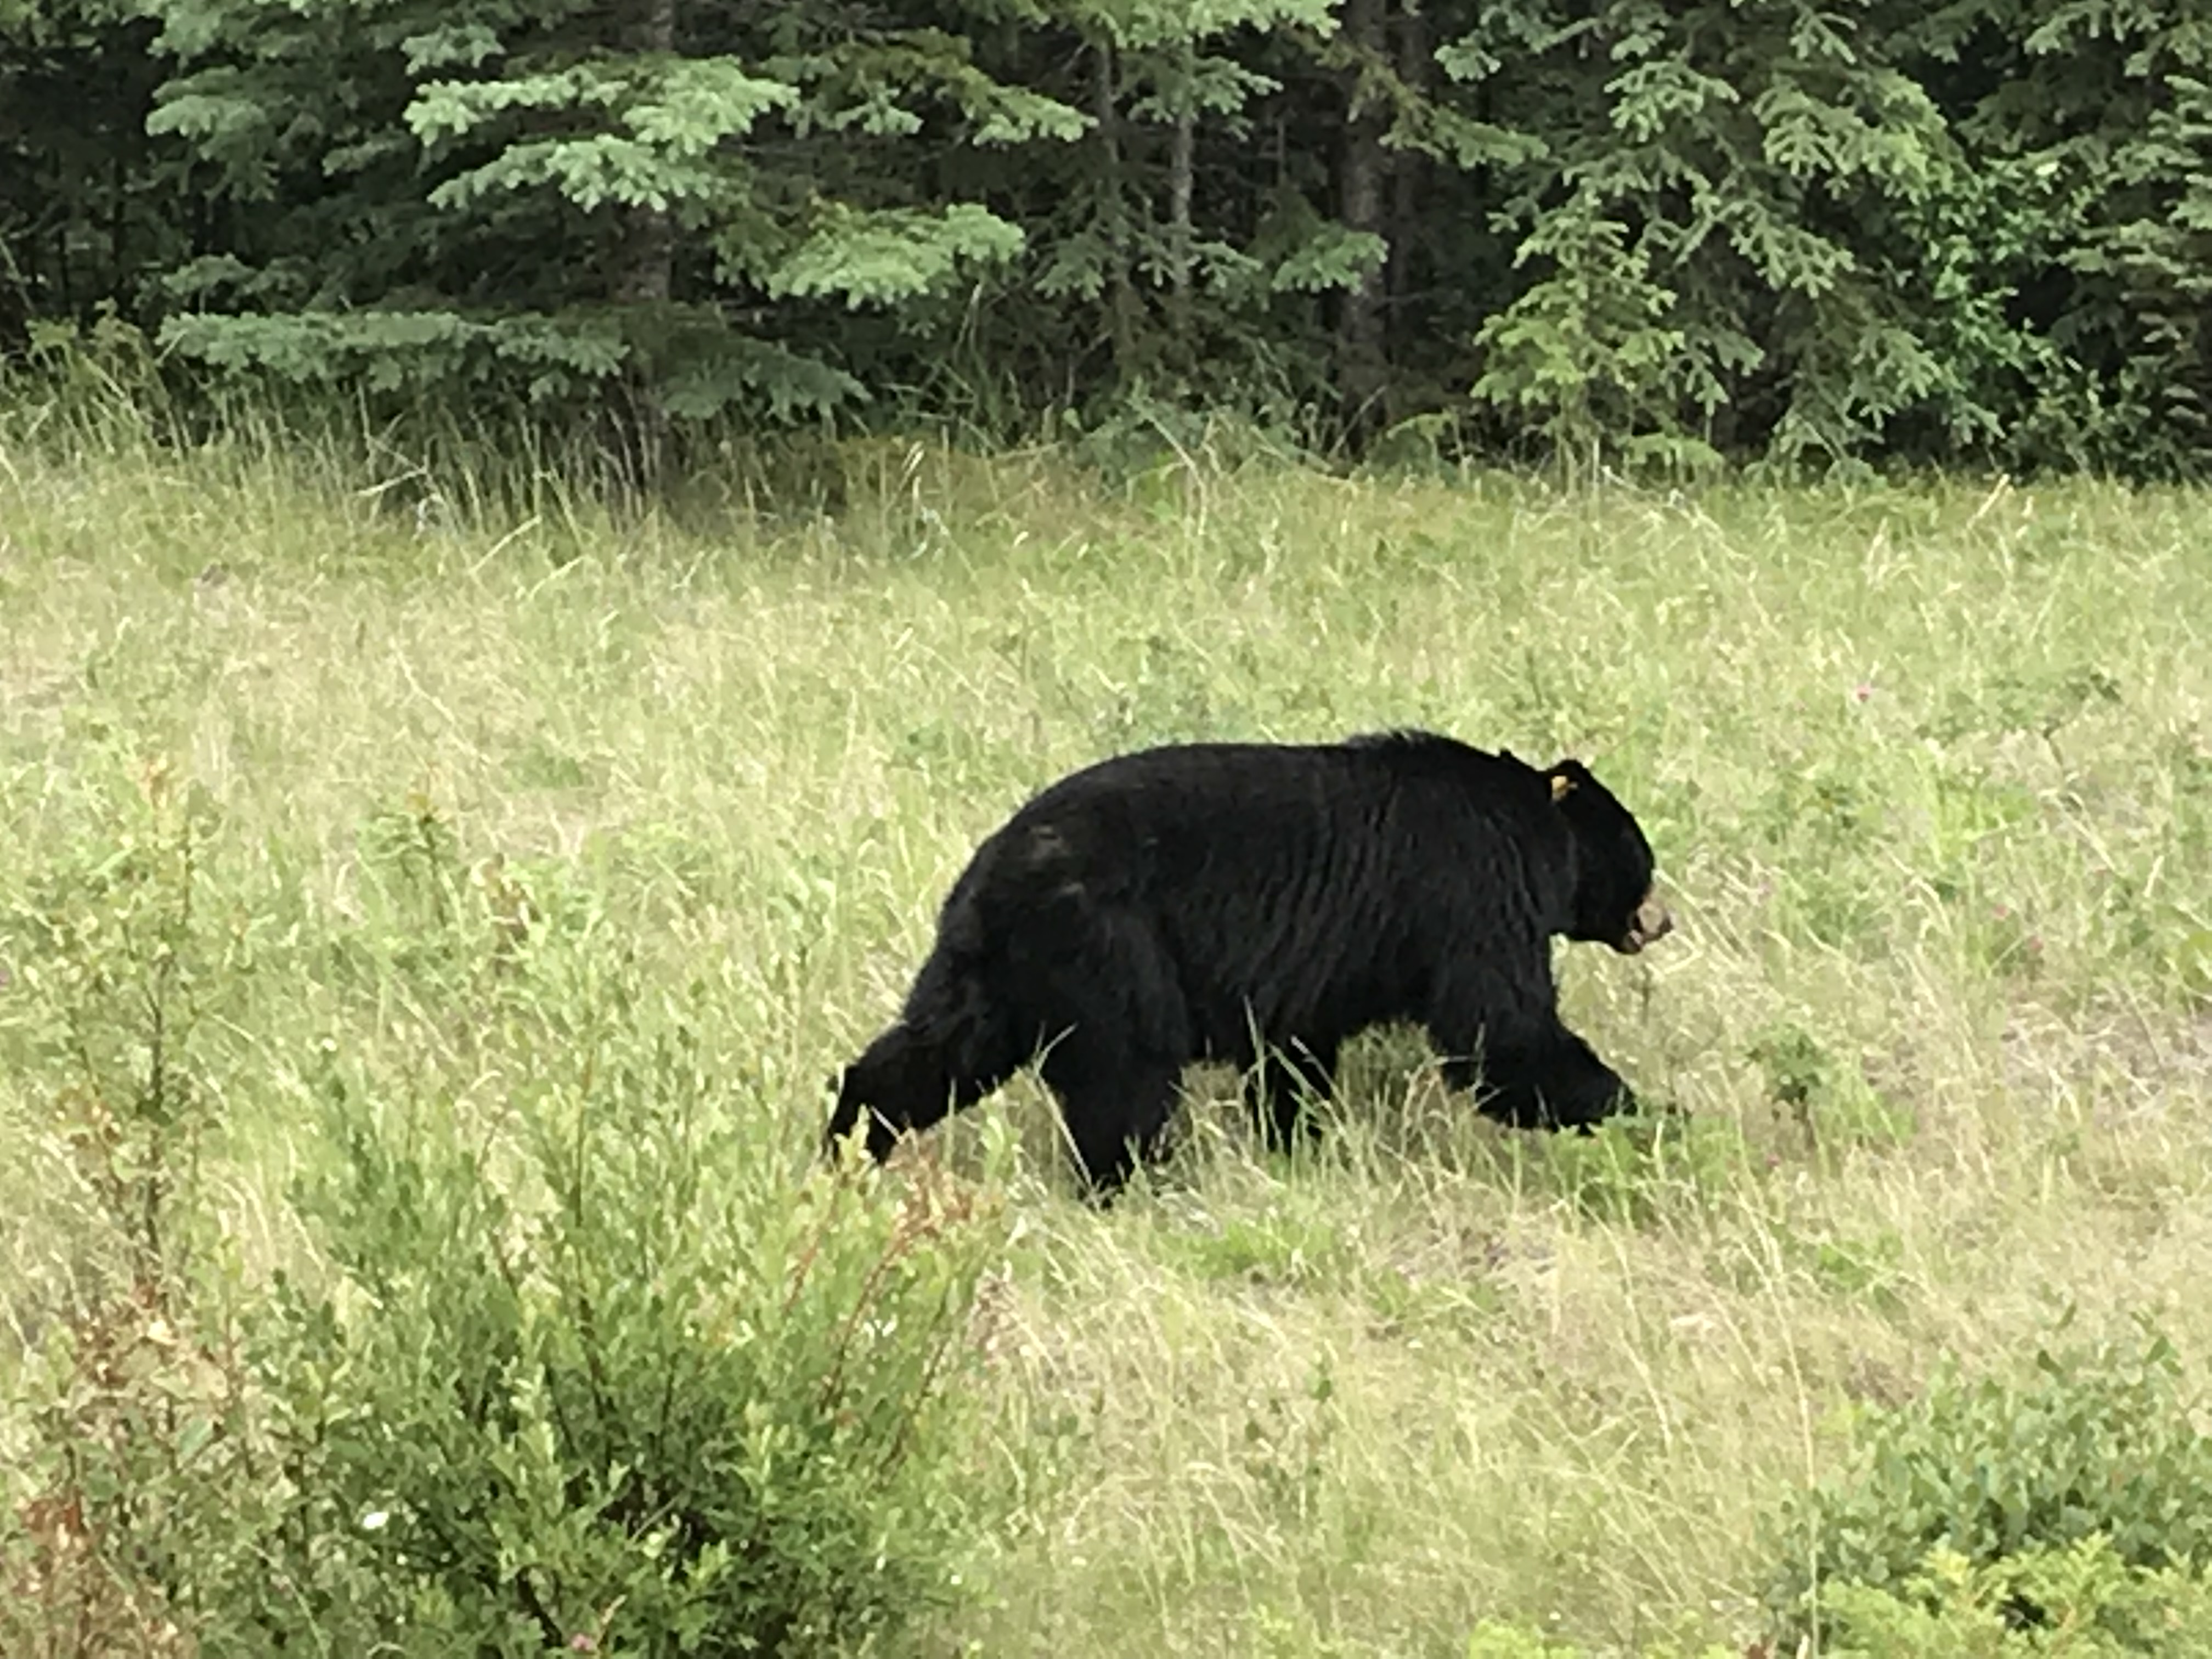
\includegraphics[height=2.5cm]{assets/jasper-black-bear.jpeg}
        \caption{A \emph{black bear} I spotted in Jasper, AB back in July 2018.}
    \end{figure}
\end{frame}

\begin{frame}
    \frametitle{Applications in Geophysics}
    \begin{itemize}
        \item Geophysicists often use waves sent from the surface to probe deep into the Earth
        \item e.g., for \emph{subsurface imaging} and \emph{earthquake predictions}
        \item These waves have both frequency and speed (how fast they travel horizontally), so the input is $(\omega, c)$
        \item There are \emph{Love waves} (``side to side,'' bandwidth $b = 1$) and \emph{Rayleigh waves} (``rolling,'' $b = 3$)
        \item The test case I use is a synthetic $100$-layer profile of each type
    \end{itemize}
    \medskip
    \begin{figure}
        \centering
        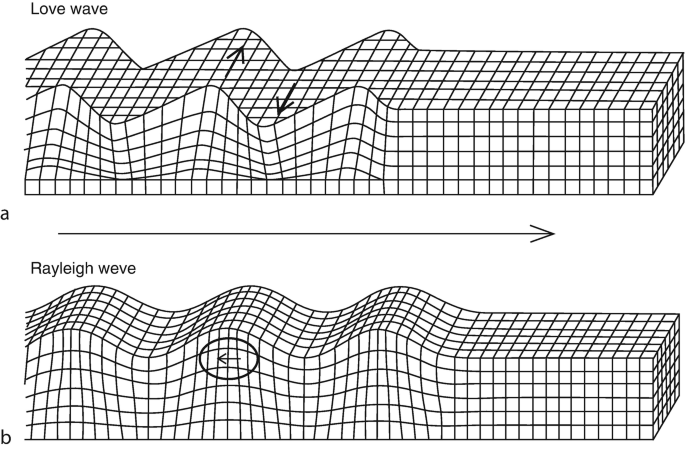
\includegraphics[height=3.5cm]{assets/love-rayleigh-waves.png}
    \end{figure}
\end{frame}

\begin{frame}
    \frametitle{Applications in Geophysics}
    Love wave stiffness matrix:\vfill
    \[
        \resizebox{\textwidth}{!}{$
        K(\omega, c) = \begin{bmatrix}
            \mu_1 \nu_1 \coth(\nu_1 h_1) & -\mu_1 \nu_1 \operatorname{csch}(\nu_1 h_1) & & \\
            -\mu_1 \nu_1 \operatorname{csch}(\nu_1 h_1) & \sum_{j = 1}^{2} \mu_j \nu_j \coth(\nu_j h_j) & \ddots & \\
            & \ddots & \ddots & -\mu_N \nu_N \operatorname{csch}(\nu_N h_N) \\
            & & -\mu_N \nu_N \operatorname{csch}(\nu_N h_N) & \mu_N \nu_N \coth(\nu_N h_N) + \mu_{N + 1} \nu_{N + 1}
        \end{bmatrix}
        $}
    \]
    \vfill
    \[
        \nu_j \coloneqq \omega \sqrt{\frac{1}{c^2} - \frac{1}{V_{s, j}^2}}
    \]
\end{frame}

\begin{frame}
    \frametitle{Applications in Geophysics}
    Rayleigh wave stiffness matrix:\vfill
    \[
        K(\omega, c) = \begin{bmatrix}
            A_1 & B_1 & & \\
            C_1 & D_1 + A_2 & \ddots & \\
            & \ddots & \ddots & B_N \\
            & & C_N & D_N + K_{N + 1}
        \end{bmatrix}
    \]
    \vfill
    \begin{gather*}
        \fitwidth{$
        k \coloneqq \omega / c, \enspace
        \gamma_j \coloneqq k^2 + s_j^2, \enspace
        r_j \coloneqq \sqrt{k^2 - \omega^2 / V_{p, j}^2}, \enspace
        s_j \coloneqq \sqrt{k^2 - \omega^2 / V_{s, j}^2},
        $} \\
        \fitwidth{$
        E_j \coloneqq \begin{bmatrix}
            ik & 0 & 0 & s_j \\
            0 & i r_j & k & 0 \\
            ik \cosh(r_j h_j) & ik \sinh(r_j h_j) & s_j \sinh(s_j h_j) & s_j \cosh(s_j h_j) \\
            i r_j \sinh(r_j h_j) & i r_j \cosh(r_j h_j) & k \cosh(s_j h_j) & k \sinh(s_j h_j)
        \end{bmatrix}, \quad
        F_j \coloneqq \mu_j \begin{bmatrix}
            0 & -2ik r_j & -\gamma_j & 0 \\
            -i \gamma_j & 0 & 0 & -2k s_j \\
            2ik r_j \sinh(r_j h_j) & 2ik r_j \cosh(r_j h_j) & \gamma_j \cosh(s_j h_j) & \gamma_j \sinh(s_j h_j) \\
            i \gamma_j \cosh(r_j h_j) & i \gamma_j \sinh(r_j h_j) & 2k s_j \sinh(s_j h_j) & 2k s_j \cosh(s_j h_j)
        \end{bmatrix},
        $} \\
        \fitwidth{$
        \begin{bmatrix}
            A_j & B_j \\
            C_j & D_j
        \end{bmatrix} \coloneqq F_j E_j^{-1}, \quad
        K_{N + 1} \coloneqq \frac{\mu_{N + 1}}{k^2 - r_{N + 1} s_{N + 1}} \begin{bmatrix}
            r_{N + 1} \bigl(k^2 - s_{N + 1}^2\bigr) & k \bigl(2 r_{N + 1} s_{N + 1} - \gamma_{N + 1}\bigr) \\
            k \bigl(2 r_{N + 1} s_{N + 1} - \gamma_{N + 1}\bigr) & s_{N + 1} \bigl(k^2 - s_{N + 1}^2\bigr)
        \end{bmatrix}
        $}
    \end{gather*}
\end{frame}

\begin{frame}
    \frametitle{Applications in Astrophysics}
    \begin{itemize}
        \item Stars \emph{oscillate} (a.k.a. ``vibrate'') at certain valid frequencies\footnote{I am a political scientist and computer scientist, \emph{not} a physicist. Despite my best friend's efforts---you should check out her talk---I do not know how to explain this. I just know the math!}\vfill
        \item This depends only on frequency, so the input is just $\omega$\vfill
        \item Measuring these frequencies lets astrophysicists\footnote{Like my awesome bestie. Seriously, she's so fed up with my cluelessness right now.} ``see'' inside a star\vfill
        \item The test case I use is $\ell = 1$ (i.e., two halves oscillate opposite each other)\footnote{My bestie vehemently insisted I ``do the hand motions'' here, so I will do so.} for the \emph{red giant HD~128279}, with bandwidth $b = 2$ \vfill
    \end{itemize}
    \begin{figure}
        \centering
        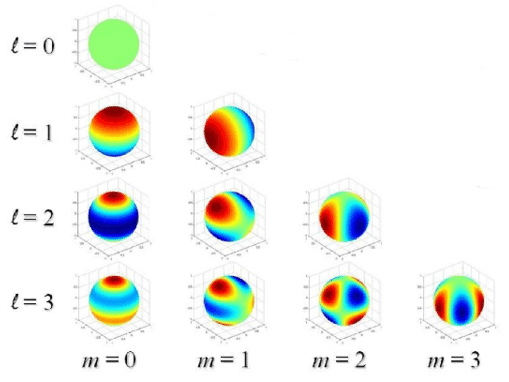
\includegraphics[height=3cm]{assets/stellar-oscillations.png}
    \end{figure}
\end{frame}

\begin{frame}
    \frametitle{Applications in Astrophysics}
    Stellar oscillation matrix (Cowling approximation):
    {
        \scriptsize
        \[
            \fitwidth{$
            K(\omega) = \begin{bmatrix}
                \omega^2 r_0 \quad -\ell / \rho_0 & & & \\
                -\bigl(I + \tfrac{h_0}{2} A_0\bigr) & I - \tfrac{h_0}{2} A_1 & & \\
                & \ddots & \ddots & \\
                & & -\bigl(I + \tfrac{h_{M - 1}}{2} A_{M - 1}\bigr) & I - \tfrac{h_{M - 1}}{2} A_M \\
                & & & -\rho_M g_M \quad 1
            \end{bmatrix}
            $}
        \]
    }
    \vfill
    \[
        A_i \coloneqq \begin{bmatrix}
            -\dfrac{2}{r_i} + \dfrac{g_i}{c_{s, i}^2} & \dfrac{1}{\rho_i c_{s, i}^2} \biggl(\dfrac{S_{\ell, i}^2}{\omega^2} - 1\biggr) \\
            \rho_i \bigl(\omega^2 - N_i^2\bigr) & -\dfrac{g_i}{c_{s, i}^2}
        \end{bmatrix}
    \]
\end{frame}

\begin{frame}
    \frametitle{Problems with Usual Methods}
    \begin{itemize}
        \item $O(nb^2)$ \emph{determinant scanning}: looks for sign changes in $\det(K)$ as input varies (most common standard)
        \begin{itemize}
            \item Two nearby modes can cancel sign changes, evading detection\vfill
            \item Does not return \emph{mode shape} (i.e., the kernel vector associated with each mode, representing how much each layer boundary moves)
        \end{itemize}\vfill
        \item $O(n^3)$ \emph{dense SVD or RRQR}: normal SVD/RRQR routines
        \begin{itemize}
            \item Numerically robust but slow
        \end{itemize}\vfill
        \item $O(nb^2)$ \emph{sparse SVD}: SVD optimized for sparse matrices
        \begin{itemize}
            \item Faster but (in theory for linear algebra reasons) may converge slower when modes are close by\footnote{I have not yet tested out sparse SVD; this project originated as a numerical linear algebra one, with the intent of developing a banded RRQR algorithm. This talk just applies the algorithm to physics cases, but it is very possible that sparse SVD is a competitive alternative.}
        \end{itemize}\vfill
    \end{itemize}
\end{frame}

\begin{frame}
    \frametitle{Banded RRQR as an Alternative}
    \begin{itemize}
        \item \emph{Rank-revealing QR} factors $KP = QR$ where $Q$ is orthonormal, $R$ is upper triangular, and $P$ reorders columns, choosing $P$ so the most linearly independent columns come first\vfill
        \item A near-zero last diagonal entry of $R$ \emph{reveals} that $K$ is singular (i.e., its producing inputs form a mode)\vfill
        \item Back-substitution gives the kernel vector or \emph{mode shape}\vfill
        \item Ordinary RRQR is $O(n^3)$, and sparse QR is only heuristically rank-revealing\vfill
        \item \emph{Banded RRQR} only pivots within the current block of columns representing one boundary's requirements, taking $O(nb^2)$ time\vfill
        \item This is done ``from both ends'' of $K$\vfill
    \end{itemize}
\end{frame}

\begin{frame}
    \frametitle{Numerical Results}
    \begin{figure}
        \centering
        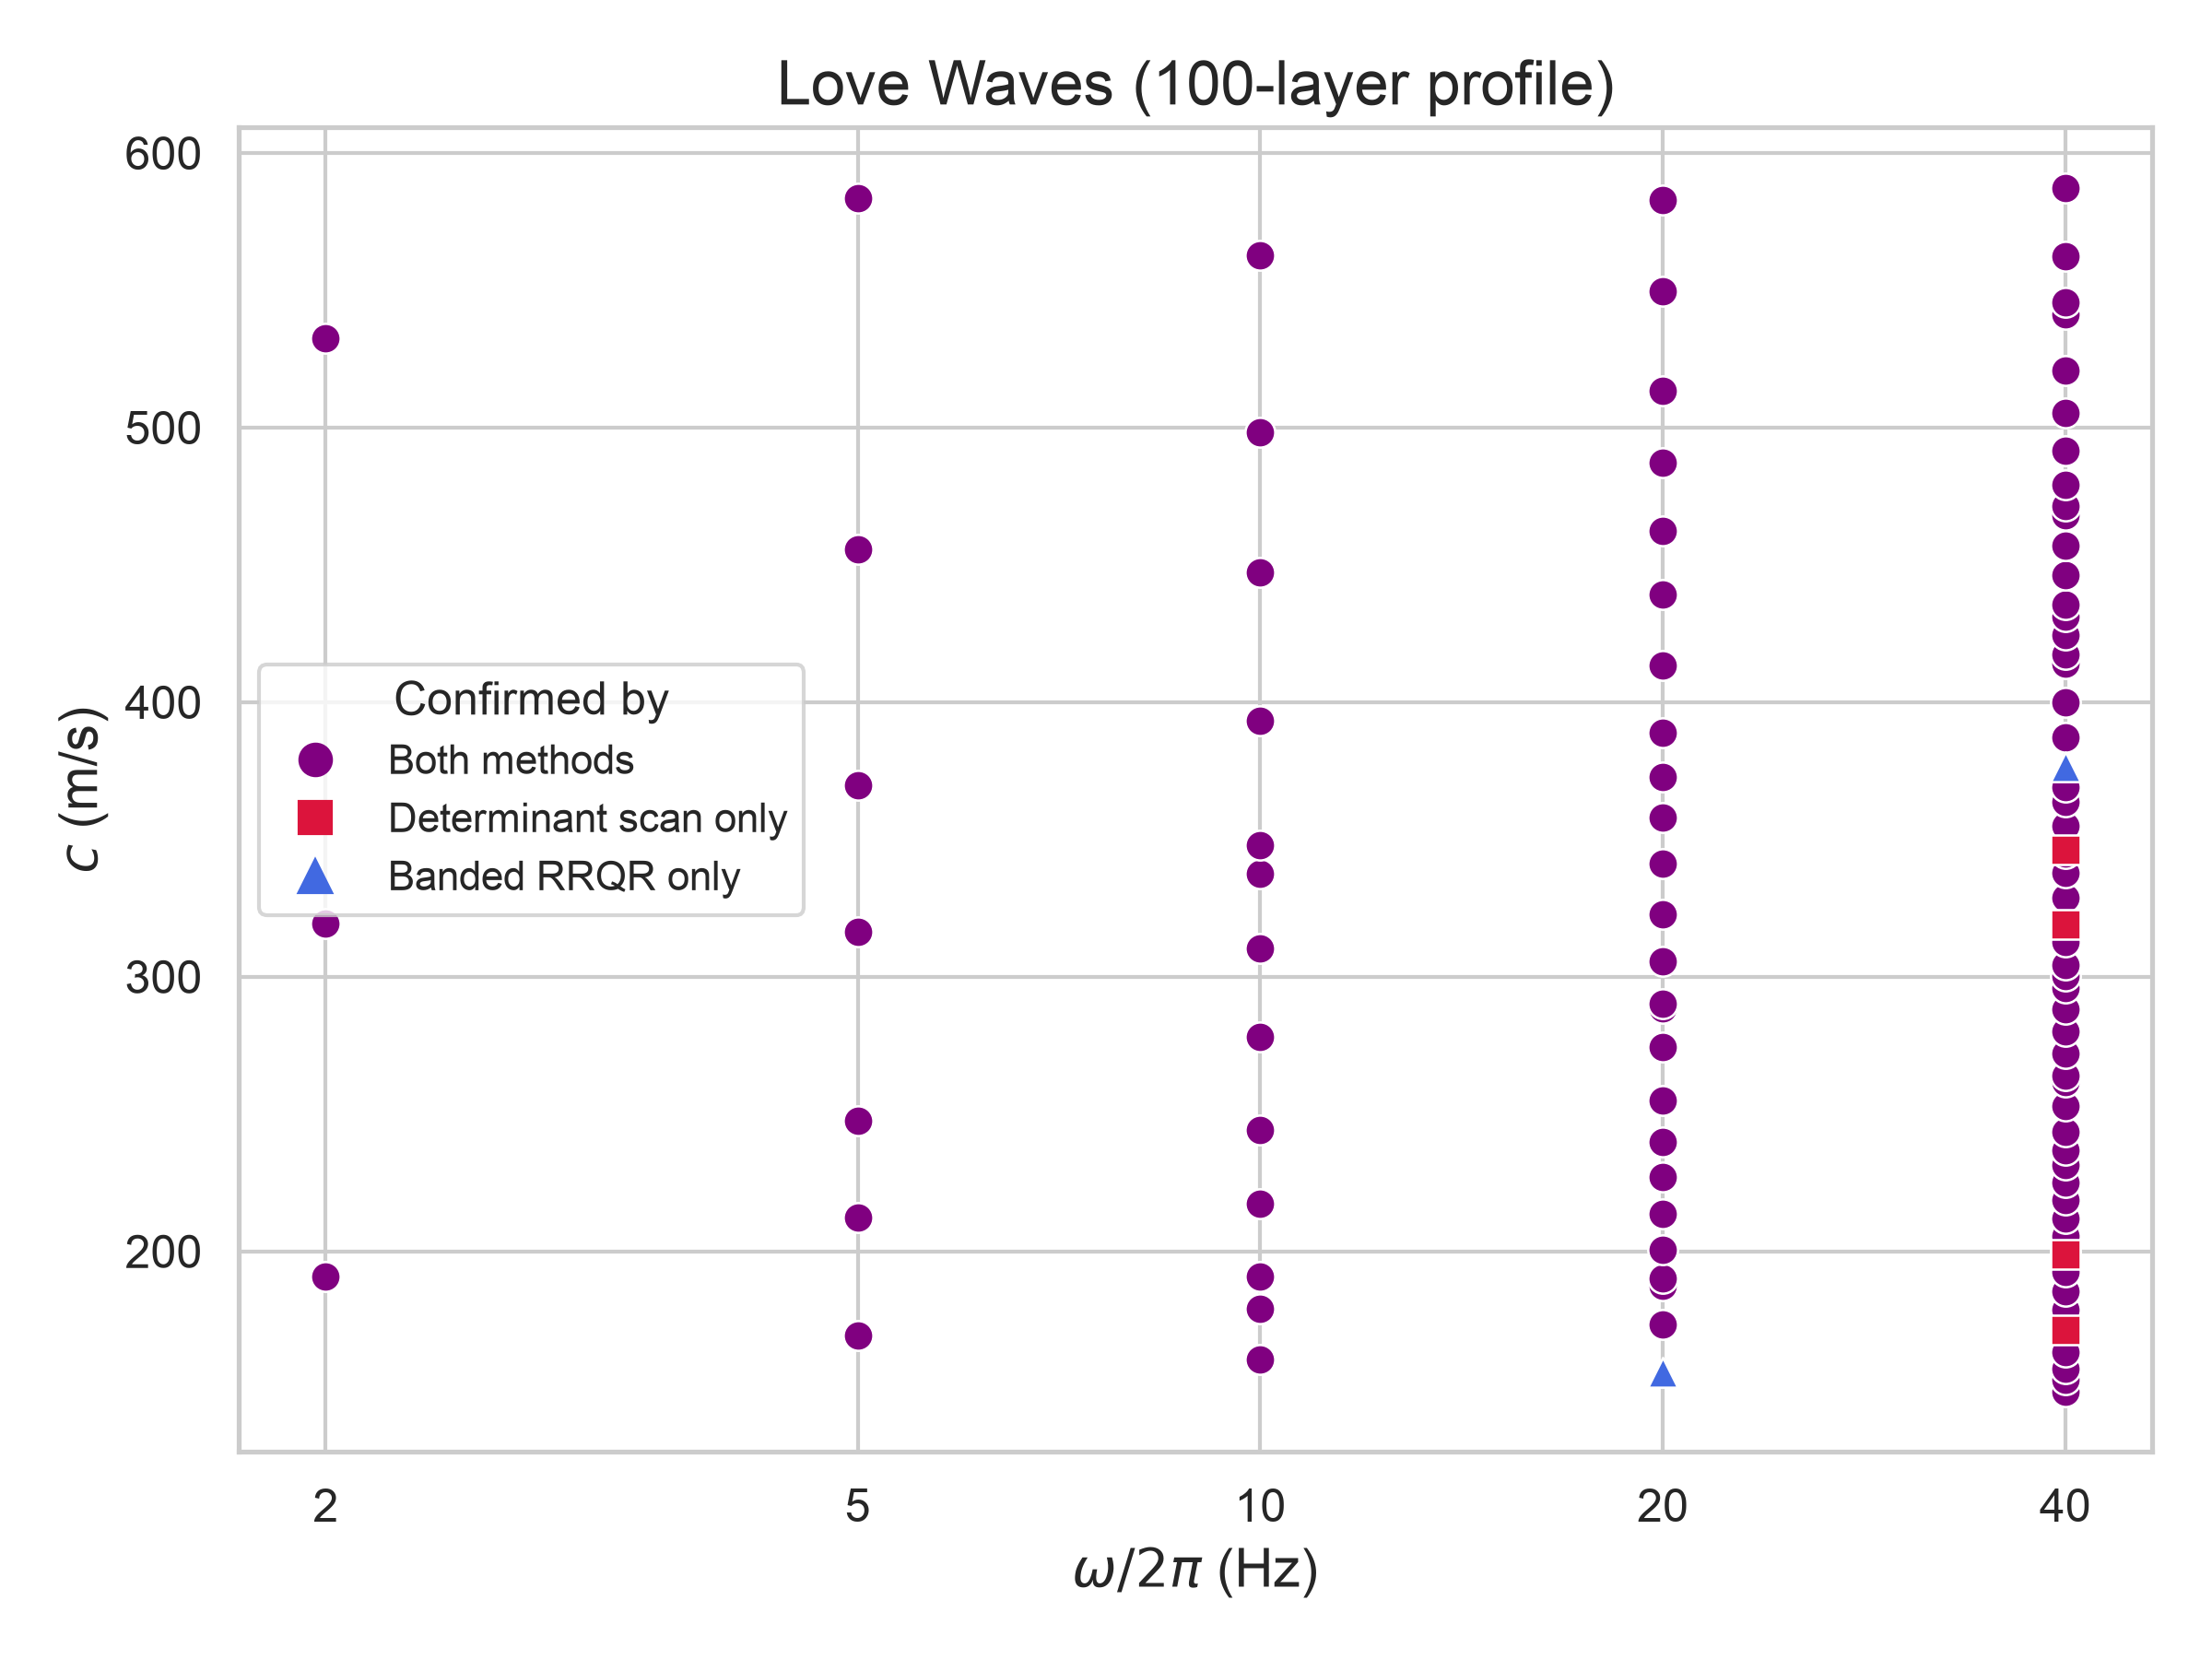
\includegraphics[width=\textwidth, height=0.7\textheight, keepaspectratio]{assets/love-modes.png}
        \caption{Banded RRQR finds 101/105 and determinant scanning finds 103/105. However, banded RRQR's misses come from ``merging'' nearby modes whereas determinant scanning misses pairs of close modes altogether.}
    \end{figure}
\end{frame}

\begin{frame}
    \frametitle{Numerical Results}
    \begin{figure}
        \centering
        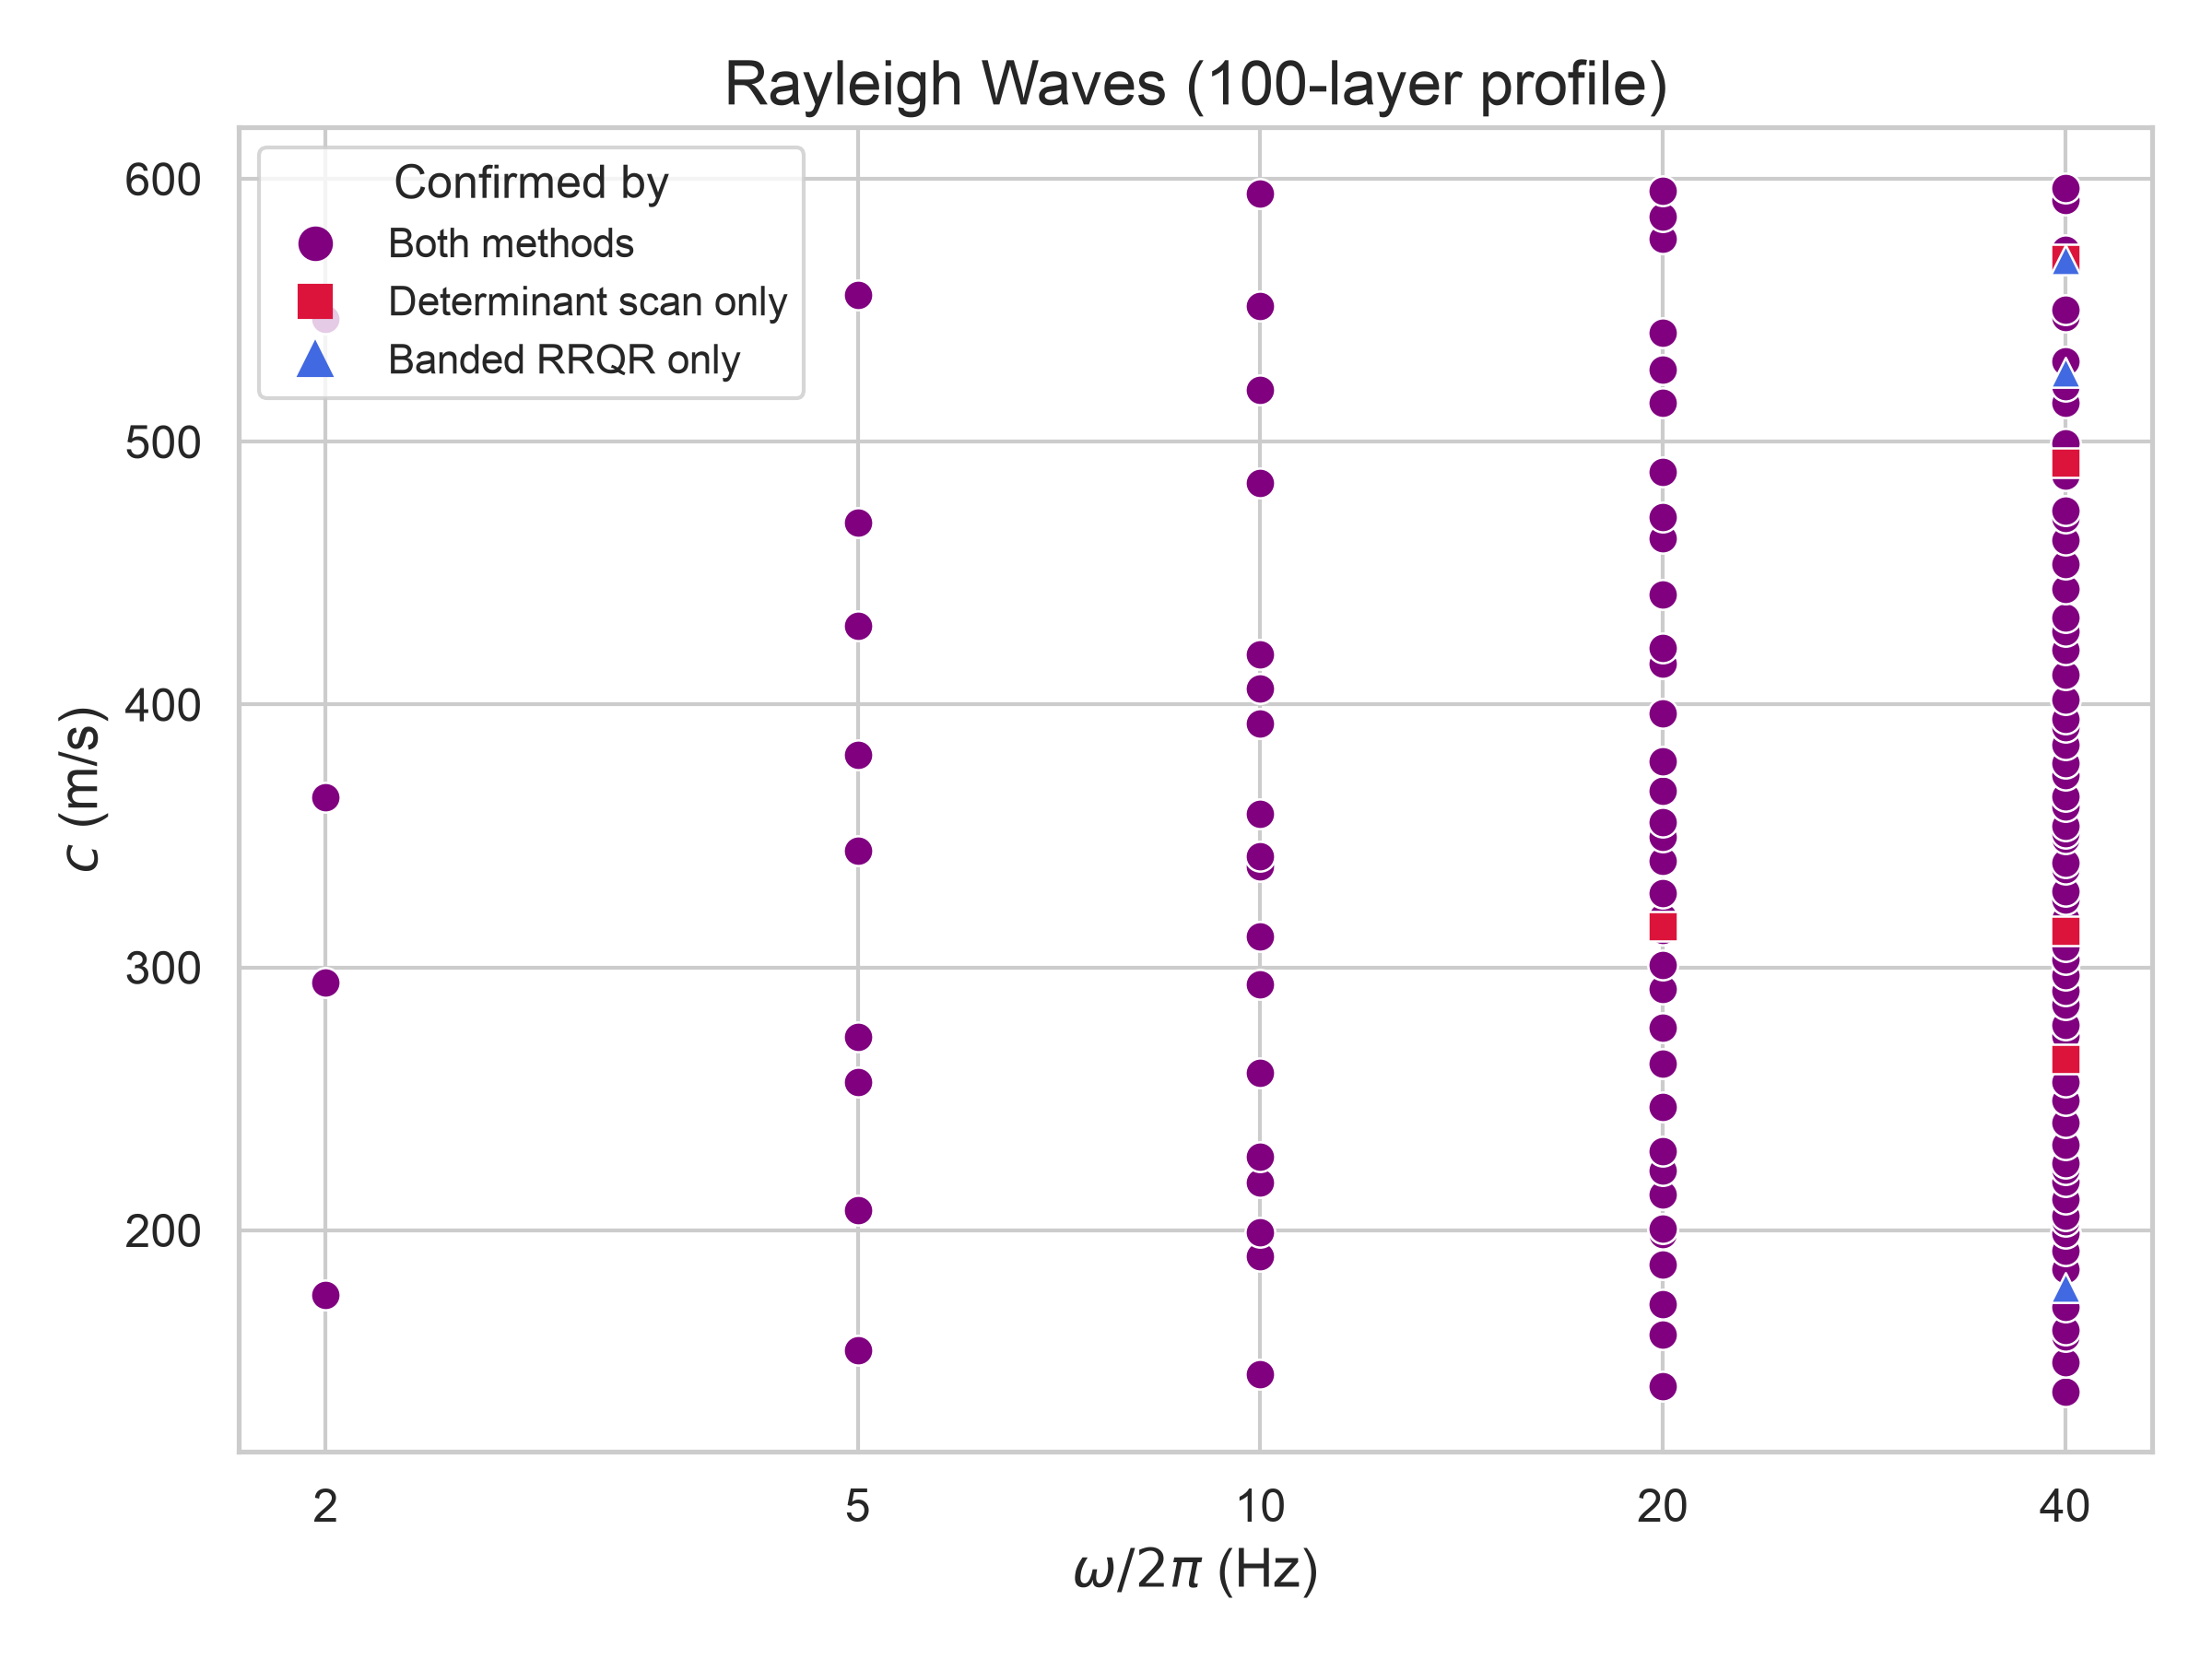
\includegraphics[width=\textwidth, height=0.7\textheight, keepaspectratio]{assets/rayleigh-modes.png}
        \caption{Again, banded RRQR finds 133/138 while determinant scanning finds 135/138, and banded RRQR ``merges'' while determinant scanning misses nearby modes entirely.}
    \end{figure}
\end{frame}

\begin{frame}
    \frametitle{Numerical Results}
    \begin{figure}
        \centering
        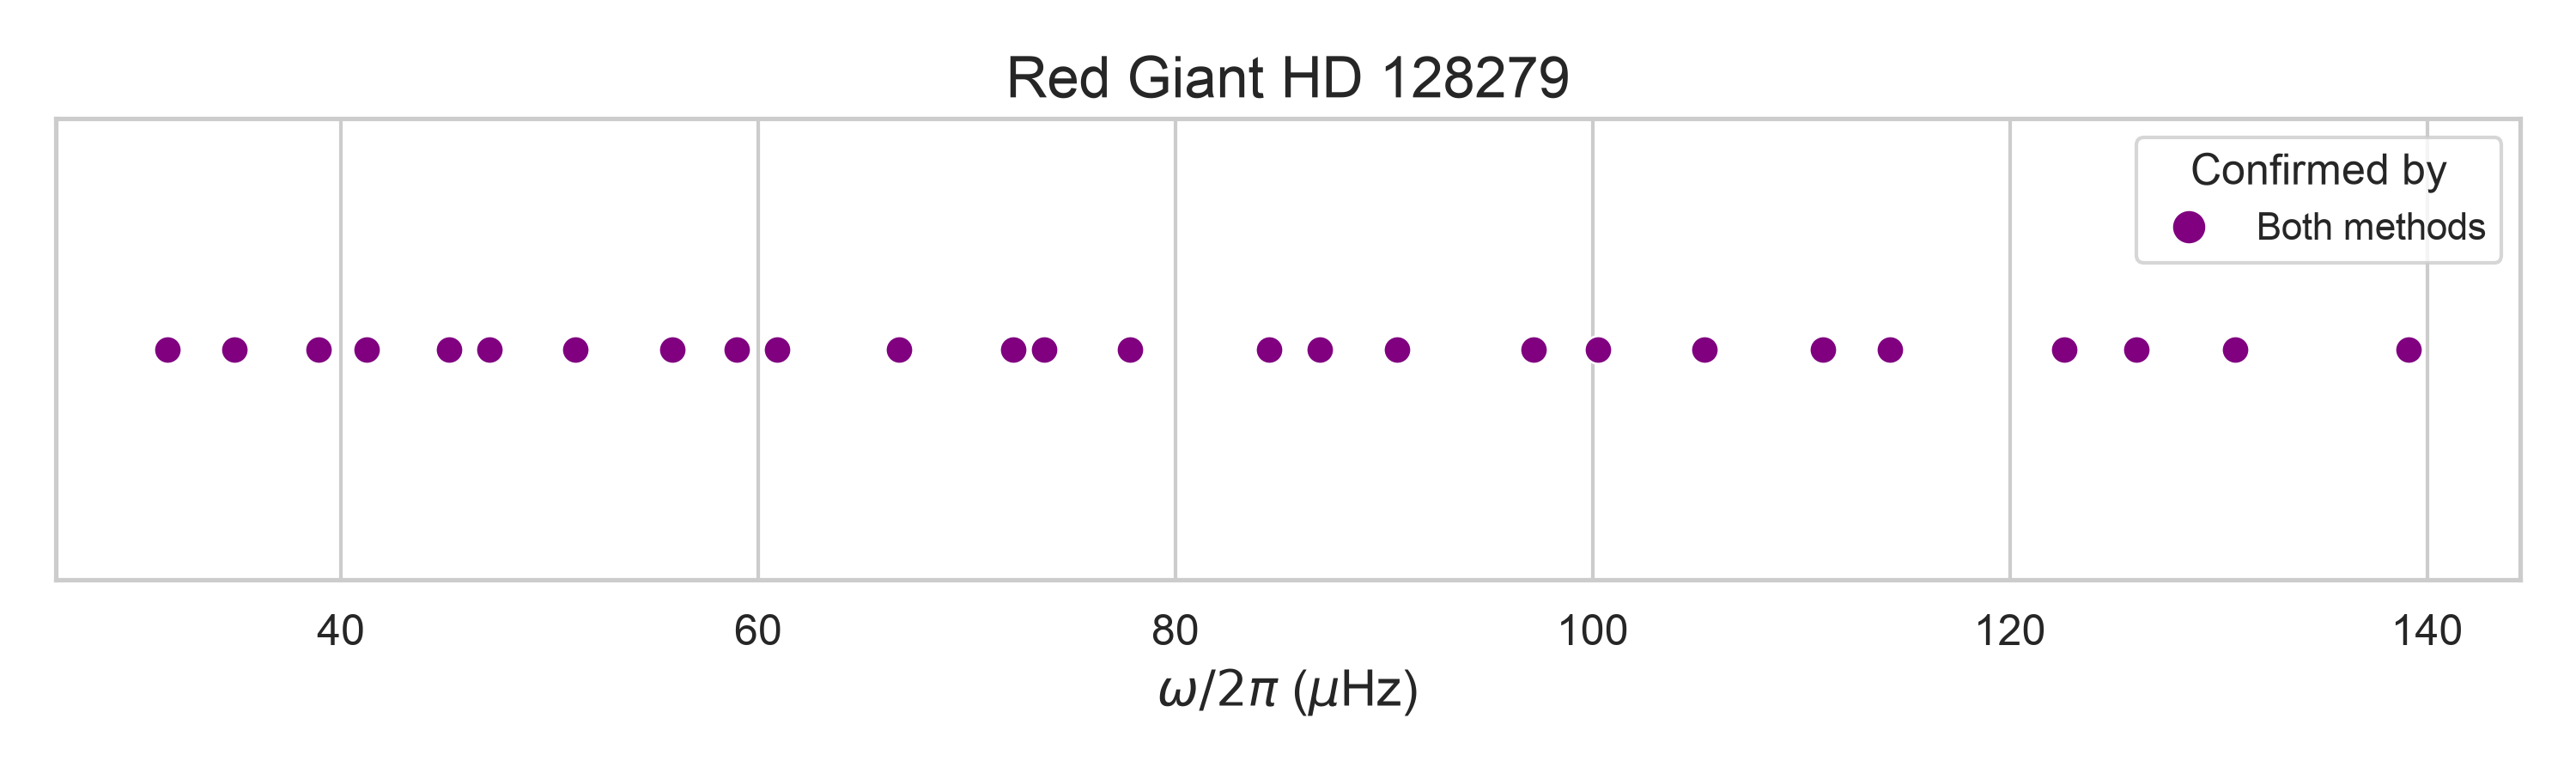
\includegraphics[width=\textwidth, height=0.65\textheight, keepaspectratio]{assets/stellar-modes.png}
        \caption{Both banded RRQR and determinant scanning find exactly 26 modes for red giant HD~128279 with $\ell = 1$.}
    \end{figure}
    \vspace*{-0.2cm}
    
\includegraphics[height=2.4cm]{assets/pusheen_reading.png}
\end{frame}

\begin{frame}
    \frametitle{Future Work}
    \begin{itemize}
        \item \emph{Damping:} Account for energy absorption in soil (right now, pretending no energy is ever lost)\vfill
        \item \emph{Other stellar oscillations:} Check, e.g., other stars or other $\ell$ parameters\vfill
        \item \emph{Stop merging:} Correctly separate nearby modes\vfill
        \item \emph{Check alternatives:} Compare directly against sparse SVD (both w.r.t. runtime and robustness of results)\vfill
        \item \emph{Further improve the algorithm:} Began primarily as a numerical analysis/algorithms project,\footnote{And on the off chance this is ever published (most of my research nowadays is in political philosophy or graph algorithms), it will be in an NA journal, not a physics one.} so focus on the actual algorithm itself\vfill
    \end{itemize}
\end{frame}

\begin{frame}
    \frametitle{Thank you for listening!}
    \begin{figure}
        \centering
        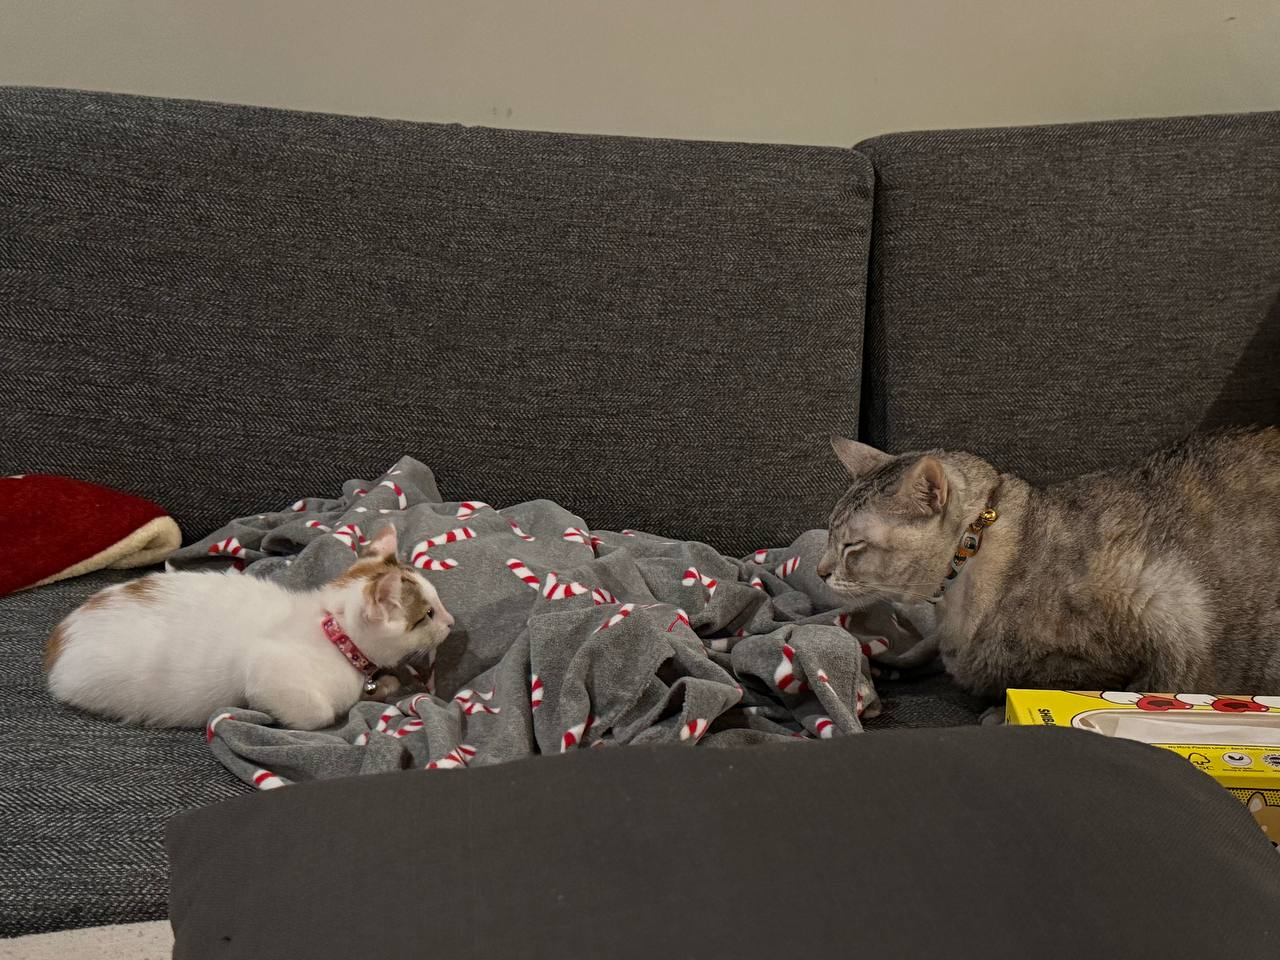
\includegraphics[height=0.77\textheight]{assets/yuki_and_ash.JPG}
        \caption{My cats, \emph{Yuki} (left) and \emph{Ash}, being sleepy and cute.}
    \end{figure}
\end{frame}

\end{document}
